\subsection{First Receipt Test}
\label{sec:eval:external_receipts}

We use SROIE receipt text and human field labels \citep{ref_sroie2019}.
A random sample selects 60 of 626 documents from the corrected trainval
mirror (seed 20260922). We join text lines in their stored order.
The model receives this text and four field names: company, date, address,
and total. The scorer reads the field labels.
One receipt has no address label, leaving 239 scored fields.
Every method is scored on these fields.
The model receives all four field names.

Gemma first extracts a graph. Three repair prompts receive this same graph
with the settings in Section~\ref{sec:impl:enhancement}.
We fix samples and settings before calling the model.
The test has 60 extraction calls and 180 repair outputs.
Each repair response is scored before and after filtering.
We also run source copying and rule repair with their original settings.
The main score uses exact triples. A second score ignores case and
whitespace in values.

\begin{table*}[t]
\centering
\caption{First SROIE test on 60 receipts. Exact match uses labelled fields. Normalized F1 ignores case and whitespace in values.}
\label{tab:external_receipts}
\small
\begin{tabular}{lrrrr}
\toprule
Method & Triple F1 & Exact match & Normalized F1 & Facts kept \\
\midrule
Extracted input & 0.7944 & 0.3333 & 0.8153 & 1.0000 \\
Rule Only & 0.7944 & 0.3333 & 0.8153 & 1.0000 \\
Source-field Copy & 0.0000 & 0.0000 & 0.0000 & 0.0000 \\
Base, raw & 0.7944 & 0.3333 & 0.8153 & 1.0000 \\
Base, gate & 0.7915 & 0.3333 & 0.8123 & 0.9944 \\
Diagnostic, raw & 0.7944 & 0.3333 & 0.8153 & 1.0000 \\
Diagnostic, gate & 0.7915 & 0.3333 & 0.8123 & 0.9944 \\
SHACL context, raw & 0.7986 & 0.3333 & 0.8194 & 1.0000 \\
SHACL context, gate & 0.7956 & 0.3333 & 0.8165 & 0.9944 \\
\bottomrule
\end{tabular}
\end{table*}

The input reaches 79.44\% F1. After filtering, base and error-report prompts
both reach 79.15\%. SHACL context reaches 79.56\%.
The error-report minus base difference is $0.00$ points
(95\% CI: $[0.00,0.00]$; paired randomization $p=1.0000$).
Field copying reaches 0.00\% F1 on receipts and 100\% on the named-field
Chinese records.

Of 239 reference values, 220 occur exactly in the source text.
The other 19 differ from the source strings.
Filtering rejects 3 candidates, all matching reference values.
They use the same address in three settings. The source has a double space;
the parser replaces it with a single space in the candidate.
After the run, we apply the same whitespace rule to the source.
All three settings then keep the address.
F1 is 79.44\% for base and error-report prompts and 79.86\% for SHACL.
Exact graph match stays at 33.33\%.
Table~\ref{tab:external_receipts} gives the original-rule scores.

The run has 240 recorded requests, including retries, and 240 parsed outputs.
Mean repair request times are 7.87, 7.92, and 8.05 seconds for base,
error-report, and SHACL prompts. Mean input lengths are 661, 715, and
2276 tokens. Request times include pacing. Extraction and context setup
are counted apart.

\begin{figure}[t]
\centering
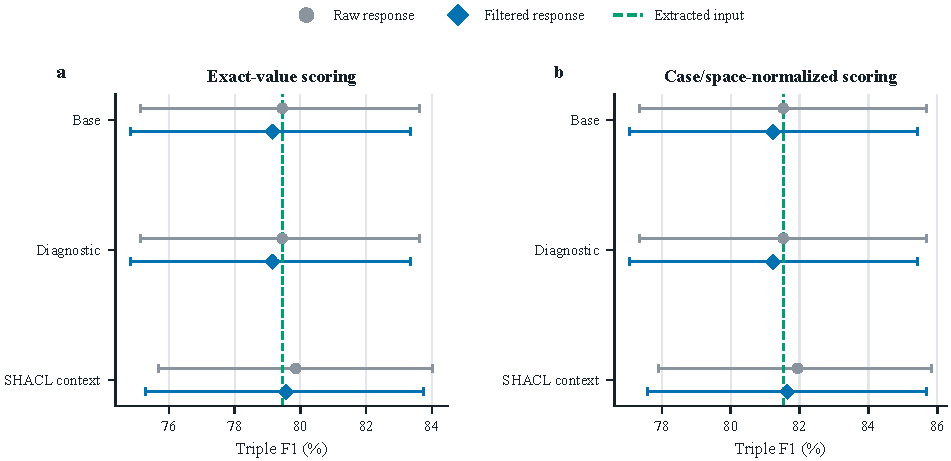
\includegraphics[width=0.98\textwidth]{figure/experiments/external_receipts.pdf}
\caption{First receipt scores. Points show mean F1 and 95\% document-bootstrap CIs. Each raw/gated pair uses one response. The dashed line shows input F1.}
\label{fig:external_receipts}
\end{figure}
